\documentclass[11pt,a4paper]{article}
\usepackage[margin=1in]{geometry}
\usepackage{hyperref}
\usepackage{enumitem}
\usepackage{graphicx}
\usepackage{xcolor}
\usepackage{booktabs}
\usepackage{longtable}
\usepackage{tikz}
\usetikzlibrary{positioning, arrows.meta}

% -----------------------------------------------------
% bvraghav-tiet-ucs503p-article.sty
% -----------------------------------------------------

% Variable: Lab Instructor
\makeatletter \newcommand{\BvrSetLabInstructor}[1]{%
  \gdef\Bvr@LabInstructor{#1}}
% default
\newcommand{\Bvr@LabInstructor}{Dr. Raghav %
  B. Venkataramaiyer}
% public accessor
\newcommand{\BvrLabInstructorValue}{\Bvr@LabInstructor}
\makeatother

% Add subtitle
\usepackage{titling}
% -- Set title bold
\pretitle{\begin{center}\bfseries\fontsize{18bp}{18bp}\selectfont}
\makeatletter
\newcommand{\BvrSubtitle}[1]{%
  \posttitle{%
    \par\end{center}
    \begin{center}\large#1\end{center}
    \vskip 0.5em}%
}
\makeatother

% Hints in the section title(s)
\newcommand{\BvrHint}[1]{%
  {\normalfont\normalsize\itshape\hfill #1}}

% -----------------------------------------------------

\title{AI-Based Student Sports Talent \& Fitness Guidance Portal}

\BvrSetLabInstructor{Dr. Raghav B. Venkataramaiyer}

\BvrSubtitle{%
  Final Project Report for UCS503P  \\
  Submitted to: \BvrLabInstructorValue \\ \bfseries
  Thapar Institute of Engineering and Technology%
}

\author{
  Kiratpreet Kaur (1024030402) \and Prisha Goyal (1024030404)
}

\date{\today}

\begin{document}
\maketitle

\section{Higher-order goal%
  \BvrHint{\ldots secondary framing}}
This project aims to help schools move from ad-hoc,
paper-based fitness records toward evidence-informed
sports guidance, so that students with genuine athletic
potential are less likely to be overlooked and students
who are interested in sport receive individualised,
data-backed direction rather than generic advice. The
broader framing -- more capable, confident young athletes
-- is treated as a secondary, motivating lens; the
primary engineering commitment remains a working,
coach-supervised assessment-to-guidance pipeline.

\section{Time-to-value %
\BvrHint{\ldots primary heuristic}}
\begin{itemize}[leftmargin=0.7cm]
    \item We delivered the core assessment-to-prediction workflow first, before any secondary feature (reporting, dashboards), so that the riskiest technical question -- can a fitness-level model be trained honestly on available data -- was answered early.
    \item We prioritised a working, if narrow, vertical slice (assessment entry $\to$ ML prediction $\to$ coach approval $\to$ student visibility) over a wide but shallow feature set.
    \item Success for this stage is defined by what is demonstrably working end-to-end today, documented honestly in Section~\ref{sec:deliverables}, rather than by what was originally planned in the proposal.
\end{itemize}

\section{Problem Statement}
Schools conduct sports activities regularly, but student
fitness and performance data is rarely recorded in a
structured, comparable way. This creates three concrete
problems, unchanged since the proposal stage and
confirmed during development:
\begin{itemize}[leftmargin=0.7cm]
    \item \textbf{Missed potential:} students with genuine athletic ability can go unnoticed without systematic, school-wide comparison of fitness data.
    \item \textbf{Generic guidance:} interested students rarely receive individualised direction on which sport suits their physical profile or what to improve.
    \item \textbf{No progress visibility:} without repeated, comparable assessments, neither the student nor the coach can tell whether training is working.
\end{itemize}

\textbf{Why this matters now:} the Khelo India fitness-test framework already gives schools a standard, low-cost battery of tests; the missing piece is a system that turns repeated test results into structured, coach-reviewed guidance rather than a one-time paper record.

\section{Proposed Solution %
\BvrHint{\ldots Software Proposition}}
\subsection{Overview}
The delivered system is a \textbf{web-based} sports
talent and fitness guidance portal with the following
components:
\begin{itemize}[leftmargin=0.7cm]
    \item \textbf{Coach assessment entry:} a coach records a student's general fitness test results (strength, endurance, flexibility, speed-agility, BMI, attendance, motivation).
    \item \textbf{ML-assisted fitness classification:} a trained classifier predicts a fitness category and a confidence score from the recorded assessment.
    \item \textbf{Coach approval workflow:} every prediction is held back from students and parents until a coach explicitly approves or overrides it.
    \item \textbf{Student/parent guidance view:} approved results, together with assessment history, are shown to the student and, at summary level, to the parent.
    \item \textbf{PDF report generation:} a downloadable summary report per student.
\end{itemize}

\subsection{Core workflow (as implemented)}
\begin{enumerate}[leftmargin=0.7cm]
    \item Coach submits a fitness assessment for a student through the web frontend.
    \item Backend validates the submission and stores it.
    \item Backend invokes the Python ML service, which returns a predicted fitness level and confidence score.
    \item Coach reviews the prediction on the coach dashboard and marks it \emph{approved} or \emph{override}.
    \item Only approved results become visible in the student and parent views, together with historical assessments for that student.
\end{enumerate}

\subsection{Deliberate scope narrowing: two-tier design}
Early in development we identified a concrete risk:
collecting every conceivable metric for every possible
sport, for every student, from day one, would make the
system too complex for a coach to realistically operate.
We therefore split the data model into two tiers:
\textbf{Tier 1 -- General Athleticism}, a single universal
fitness battery applied to every student and used to
recommend suitable sports, which is the complete scope of
the current semester; and \textbf{Tier 2 -- Sport-Specific
KPIs}, a small, per-sport indicator set applied only to
students who are funnelled into a specific sport squad,
explicitly deferred to future work (Section~\ref{sec:deliverables}).

\section{Solution Approach %
\BvrHint{\ldots Engineering focus}}
As an engineering course project, the emphasis throughout
was on correctness, honest evaluation, and workflow
design, rather than on novel algorithms.

\subsection{Fitness classification %
\BvrHint{\ldots non-research}}
Fitness-level prediction uses standard, explainable
models rather than research-grade architectures:
\begin{itemize}[leftmargin=0.7cm]
    \item A Random Forest classifier, trained with SMOTE oversampling to address class imbalance, chosen specifically because its decisions can be inspected and explained to a non-technical coach.
    \item A leakage-control step was applied before any accuracy figure was trusted: an initial model that included a derived ``overall performance'' column reached a suspicious 98\% accuracy by relying on that column instead of genuine fitness signals; removing such columns produced a more credible, believable model.
    \item The model is shown to the user only as decision support: a coach must approve or override every prediction before it is acted on.
\end{itemize}

\subsection{Web architecture %
\BvrHint{\ldots web-based solution}}
A 3-tier web architecture, shown in Figure~\ref{fig:architecture}:
\begin{itemize}[leftmargin=0.7cm]
    \item \textbf{Frontend:} React/Vite interface for coach, student, parent, and admin views.
    \item \textbf{Backend API:} Node.js/Express, handling validation, persistence, and orchestration of the ML service.
    \item \textbf{ML service:} a Python/scikit-learn prediction script invoked by the backend per assessment.
    \item \textbf{Data store:} designed around a normalised PostgreSQL schema (Section~\ref{sec:scalability}); the current implementation persists assessments in a flat structure as an interim step.
\end{itemize}

\begin{figure}[h]
\centering
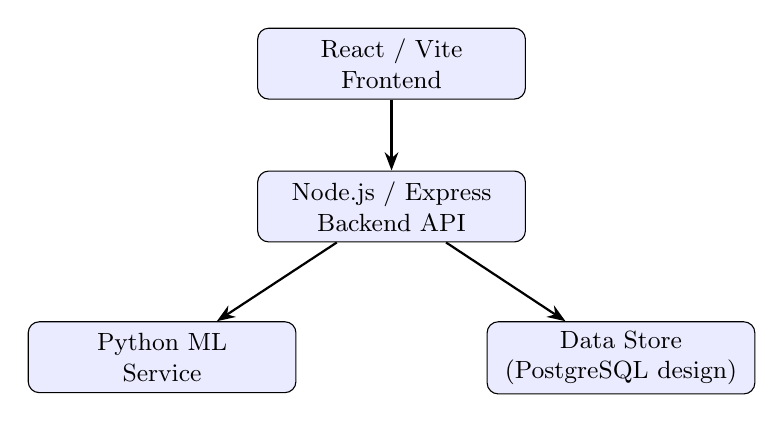
\begin{tikzpicture}[
    box/.style={draw, rounded corners, minimum width=3.4cm, minimum height=0.9cm, align=center, fill=blue!8, font=\small},
    arrow/.style={-Stealth, thick}
]
\node[box] (frontend) {React / Vite\\Frontend};
\node[box, below=0.9cm of frontend] (backend) {Node.js / Express\\Backend API};
\node[box, below left=1cm and -0.5cm of backend] (ml) {Python ML\\Service};
\node[box, below right=1cm and -0.5cm of backend] (db) {Data Store\\(PostgreSQL design)};
\draw[arrow] (frontend) -- (backend);
\draw[arrow] (backend) -- (ml);
\draw[arrow] (backend) -- (db);
\end{tikzpicture}
\caption{Implemented system architecture}
\label{fig:architecture}
\end{figure}

\subsection{Iteration and delivery}
Development proceeded in short, working increments: the
assessment-entry and BMI-calculation module was completed
and tested before the ML service was integrated; the ML
service was validated in isolation (including the
leakage-detection exercise above) before being wired into
the backend; and the coach-approval gate was added and
tested before student/parent views were connected to it.
This ordering meant that at every stage there was a
working, demonstrable slice of the system, rather than
several half-finished components.

\section{Evaluation Criterion %
\BvrHint{\ldots measurable and attributable}}
As proposed, we define success using measurable,
attributable metrics tied to the core workflow, and we
report the actual measured values rather than targets
alone.

\subsection{Primary evaluation metric}
\textbf{Classification quality on a held-out test set.}
\begin{itemize}[leftmargin=0.7cm]
    \item \textbf{Result:} 83\% overall accuracy, macro-averaged F1-score of 0.56, on a 100-record held-out test split (80/20 split of 500 records).
    \item \textbf{Attribution:} measured directly via \texttt{scikit-learn}'s classification report and confusion matrix on the trained pipeline; figures were independently re-run and confirmed rather than taken on trust from an earlier draft.
    \item \textbf{Honest limitation:} the High Performer class (12 of 500 records) was correctly identified 0 times in the test set, even with SMOTE and balanced class weights -- a genuine data-availability limitation, reported here rather than masked by the relatively high overall accuracy.
\end{itemize}

\subsection{Secondary evaluation metrics}
\begin{itemize}[leftmargin=0.7cm]
    \item \textbf{Workflow integrity:} a prediction is verified to be inaccessible to the student/parent view until a coach approval action is recorded, tested via an end-to-end integration test of Assessment $\to$ ML $\to$ Approval $\to$ Visibility.
    \item \textbf{Role isolation:} each of the four roles (Student, Coach, Admin, Parent) was verified to access only its intended views.
    \item \textbf{Explainability:} every stored prediction carries its confidence score, so no recommendation is presented as an unexplained black-box output.
\end{itemize}

\subsection{Pilot validation plan}
\begin{itemize}[leftmargin=0.7cm]
    \item A small-scale internal test used synthetic and openly available student fitness records rather than real school data, consistent with the project's data-privacy constraints for a student prototype.
    \item Coach-facing usability (can a coach complete an assessment and review a recommendation without guidance) was checked informally during development and is proposed as the basis for a future formal pilot once real coach users are available.
\end{itemize}

\section{Scalability %
\BvrHint{\ldots with foresight}}
\label{sec:scalability}
\begin{enumerate}[leftmargin=0.7cm]
    \item \textbf{Scalable (theoretically):} the system is designed around a normalised relational schema (\texttt{Students}, \texttt{Assessments}, \texttt{Coaches}, \texttt{Recommendations}, \texttt{Admins}) so that a school-wide cohort, assessed repeatedly over time, can be queried efficiently rather than requiring a redesign as data volume grows. The schema is deliberately additive: a future \texttt{Sport\_Specific\_Metrics} table for Tier~2 can be introduced without modifying the Tier~1 tables.
    \item \textbf{Operationally deployable (practically):} the frontend, backend, and ML service are decoupled and independently deployable (e.g. Vercel for the frontend, a Node-compatible host for the backend), and the ML service is invoked as a stateless per-request call, avoiding a persistent, hard-to-scale ML process.
\end{enumerate}

\section{Engine availability heuristic}
This project deliberately relies on mature, off-the-shelf
engines rather than custom infrastructure, consistent with
the course's non-research framing:
\begin{itemize}[leftmargin=0.7cm]
    \item \textbf{Web framework:} Express (REST API) and React (frontend), both mature, widely documented.
    \item \textbf{ML library:} scikit-learn and imbalanced-learn, rather than a custom-built model or training loop.
    \item \textbf{Database engine:} PostgreSQL, a mature relational engine, chosen specifically because the data is inherently relational (repeated assessments per student).
    \item \textbf{Report generation:} standard client-side PDF generation rather than a custom document-rendering pipeline.
\end{itemize}
Using these mature components let the team focus on
workflow correctness, leakage-aware evaluation, and the
coach-approval design, rather than on infrastructure that
already exists in well-tested form elsewhere.

\section{Project scope and deliverables %
\BvrHint{\ldots incremental, results over intentions}}
\label{sec:deliverables}

\subsection{Delivered in this stage}
\begin{itemize}[leftmargin=0.7cm]
    \item Coach assessment entry with automatic BMI calculation.
    \item Trained and evaluated fitness-level classifier (Random Forest with SMOTE), including a documented leakage-detection and correction process.
    \item Coach approval/override workflow, enforced before student or parent visibility.
    \item Student dashboard showing approved recommendations and assessment history.
    \item Parent dashboard showing a summary-level, coach-approved view.
    \item Downloadable PDF fitness report.
\end{itemize}

\subsection{Not yet delivered, and why}
In the spirit of reporting results rather than
intentions, the following gaps are stated plainly rather
than implied as complete:
\begin{itemize}[leftmargin=0.7cm]
    \item \textbf{Sport-suitability recommendation logic} (mapping a fitness profile to specific suggested sports) is specified but not yet implemented; the current system predicts a fitness category only.
    \item \textbf{Relational database migration:} assessments are currently persisted in a flat structure rather than the normalised PostgreSQL schema described in Section~\ref{sec:scalability}; this is the next planned increment.
\end{itemize}

\subsection{Subsequent deliverables (Tier 2 and beyond)}
\begin{itemize}[leftmargin=0.7cm]
    \item Sport-specific KPI tracking for squad-selected students, added one sport at a time.
    \item A progression/forecasting model comparing a student's improvement trajectory against age-group benchmarks.
    \item A larger, more representative dataset, particularly to make the High Performer category reliably predictable.
\end{itemize}

\section{Risks and mitigations}
\begin{itemize}[leftmargin=0.7cm]
    \item \textbf{Overtrusting model accuracy:} mitigated by the explicit leakage-detection exercise (Section 5.1) and by reporting per-class, not just overall, metrics.
    \item \textbf{Data privacy / consent:} mitigated by using only synthetic or openly available fitness data during development; no real student-identifying data was collected.
    \item \textbf{Coach adoption:} mitigated by keeping assessment entry to a single form with automatic BMI calculation, and by never surfacing an unreviewed prediction to a student or parent.
    \item \textbf{Scope creep from sport-specific tracking:} mitigated directly by the two-tier design (Section 4.3), which confines the current semester to a single, universal fitness battery.
\end{itemize}

\section{Summary}
This report documents the transition of the AI-Based
Student Sports Talent \& Fitness Guidance Portal from a
proposal to a working system. The core assessment-to-
guidance workflow -- coach entry, ML-assisted fitness
classification, mandatory coach approval, and
student/parent visibility -- is implemented and tested end
to end, and the underlying classifier was evaluated
honestly, including a documented leakage-detection process
and an explicit acknowledgement of its class-imbalance
limitation. Sport-specific recommendation logic and full
relational persistence remain the immediate next steps,
and are reported here as open work rather than implied as
complete. The project continues to meet the course's
selection criteria by favouring working increments over a
wide but shallow feature set, using mature, off-the-shelf
engines rather than research-grade components, and
defining success through measurable, attributable
evaluation criteria rather than subjective impressions of
progress.

\end{document}
